\renewcommand\chaptername{LAMPIRAN}
\label{lampiranisntalasihalamanlogin}
\chapter{Lampiran Halaman \textit{Login}}
\section{Pemasangan Perangkat Lunak}
Berikut adalah perangkat lunak yang dibutuhkan agar halaman \textit{login} dapat digunakan, antara lain:
\begin{enumerate}
	\item \textit{Python} versi 3.5.2.
	\item \textit{Flask} versi 1.0.2.
	\item \textit{Gunicorn} versi 19.8.1.
	\item \textit{Supervisor} versi 3.2.0.
	\item \textit{Nginx} versi 1.10.3.
\end{enumerate}

\subsection{Pemasangan Perangkat Lunak Python}
Berikut adalah langkah-langkah untuk memasang perangkat lunak Python versi 3.5.2 pada \textit{server} yang akan digunakan untuk membangun halaman \textit{login}.\\
\begin{minipage}{\linewidth}
	\begin{lstlisting}[caption=Command untuk installasi Python,language=Python,label=installpython3diserverlogin]
	sudo apt-get update
	sudo apt-get install python3
	\end{lstlisting}
\end{minipage}

\subsection{Pemasangan Perangkat Lunak Flask}
Berikut adalah langkah-langkah untuk memasang perangkat lunak Flask versi 1.0.2 pada \textit{server} yang akan digunakan untuk membangun halaman \textit{login}.\\
\begin{minipage}{\linewidth}
	\begin{lstlisting}[caption=Command untuk installasi Flask,language=Python,label=installflaskdiserverlogin]
	sudo apt-get install python3-pip
	sudo pip install flask
	\end{lstlisting}
\end{minipage}

\subsection{Pemasangan Perangkat Lunak Gunicorn}
Berikut adalah langkah-langkah untuk memasang perangkat lunak Gunicorn versi 19.8.1 pada \textit{server} yang akan digunakan untuk membangun halaman \textit{login}.\\
\begin{minipage}{\linewidth}
 	\begin{lstlisting}[caption=Command untuk installasi Gunicorn,language=Python,label=installgunicorndiserverlogin]
 	sudo pip install gunicorn
 	\end{lstlisting}
\end{minipage}

\subsection{Pemasangan Perangkat Lunak Supervisor}
Berikut adalah langkah-langkah untuk memasang perangkat lunak Supervisor versi 3.2.0 pada \textit{server} yang akan digunakan untuk membangun halaman \textit{login}.\\
\begin{minipage}{\linewidth}
 	\begin{lstlisting}[caption=Command untuk installasi Supervisor,language=Python,label=installsupervisordiserverlogin]
 	sudo apt-get install python-setuptools
 	sudo apt-get install supervisor
 	\end{lstlisting}
\end{minipage}

\subsection{Pemasangan Perangkat Lunak Nginx}
Berikut adalah langkah-langkah untuk memasang perangkat lunak Nginx versi 1.10.3 pada \textit{server} yang akan digunakan untuk membangun halaman \textit{login}.\\
\begin{minipage}{\linewidth}
 	\begin{lstlisting}[caption=Command untuk installasi Nginx,language=Python,label=installnginx]
 	sudo apt-get install nginx
 	\end{lstlisting}
\end{minipage}

\section{Konfigurasi Perangkat Lunak}
Beberapa perangkat lunak pada \textit{server} yang akan digunakan untuk membangun halaman \textit{login} harus dikonfigurasi terlebih dahulu agar dapat digunakan.

\subsection{File Konfigurasi Supervisor}
Berikut adalah file konfigurasi keseluruhan untuk perangkat lunak Supervisor pada \texttt{/etc/supervisor/conf.d/app.conf}.\\

\begin{minipage}{\linewidth}
	\begin{lstlisting}[caption=Konfigurasi tambahan Supervisor,language=Python,label=konfigurasisupervisor]
	[program:flask-loginpage]
	
	command = 
	/home/fourirakbar/flask-loginpage/flask-loginpageenv/bin/python 
	/home/fourirakbar/flask-loginpage/flask-loginpageenv/bin/gunicorn 
	-b 0.0.0.0:400 app:app
	directory = /home/fourirakbar/flask-loginpage
	user = fourirakbar
	stdout_logfile = 
	/home/fourirakbar/flask-loginpage/logs/app_stdout.log
	stderr_logfile =
	/home/fourirakbar/flask-loginpage/logs/app_stderr.log
	redirect_stderr = True
	autostart = True
	enviroment = PATH = 
	"/home/fourirakbar/flask-loginpage/flask-loginpageenv/bin", 
	PRODUCTION=1
	\end{lstlisting}
\end{minipage}

\subsection{File Konfigurasi Nginx}

Berikut adalah file konfigurasi keseluruhan untuk perangkat lunak Nginx pada \texttt{/etc/nginx/sites-available/app}.\\
  
  \begin{lstlisting}[numbers=left, frame=single,tabsize=2,breaklines,caption={Konfigurasi tambahan untuk Nginx},label=konfigurasinginx, language=python]

	server {
		listen 80;
		server_name 10.151.36.120;
		
		add_header X-Frame-Options SAMEORIGIN;
		add_header X-Content-Type-Options nosniff;
		add_header X-XSS-Protection "1; mode=block";
		
		access_log /home/fourirakbar/flask-loginpage/logs/app_access.log;
		
		location / {
			proxy_pass       http://127.0.0.1:4000;
			proxy_set_header Host        $host;
			proxy_set_header X-Real-IP   $remote_addr;
			proxy_set_header X-Forwarded-For $proxy_add_x_forwarded_for;
		}
		
		location ^~ /static/  {
			include     /etc/nginx/mime.types;
			alias       /home/fourirakbar/flask-loginpage/static/;
		}  
	}

\end{lstlisting}

\chapter{Lampiran Middleware}
\section{Pemasangan Perangkat Lunak}

Berikut adalah perangkat lunak yang dibutuhkan agar \textit{middleware} dapat digunakan, antara lain:
\begin{enumerate}
	\item \textit{Python} versi 3.5.2.
	\item \textit{Flask} versi 1.0.2.
	\item \textit{Docker} versi 1.13.1.
\end{enumerate}

\subsection{Pemasangan Perangkat Lunak Python}
Berikut adalah langkah-langkah untuk memasang perangkat lunak Python versi 3.5.2 pada \textit{docker host} yang akan digunakan untuk membangun \textit{middleware}.\\
\begin{minipage}{\linewidth}
	\begin{lstlisting}[caption=Command untuk installasi Python,language=Python,label=installpython3diserverlogin]
	sudo apt-get update
	sudo apt-get install python3
	\end{lstlisting}
\end{minipage}

\subsection{Pemasangan Perangkat Lunak Flask}
Berikut adalah langkah-langkah untuk memasang perangkat lunak Flask versi 1.0.2 pada \textit{docker host} yang akan digunakan untuk membangun \textit{middleware}.\\
\begin{minipage}{\linewidth}
	\begin{lstlisting}[caption=Command untuk installasi Flask,language=Python,label=installflaskdiserverlogin]
	sudo apt-get install python3-pip
	sudo pip install flask
	\end{lstlisting}
\end{minipage}




\backmatter % Lampiran tanpa judul LAMPIRAN X, biasanya untuk BIODATA PENULIS
	\chapter{BIODATA PENULIS}
		\begin{wrapfigure}{l}{0.3\textwidth}
			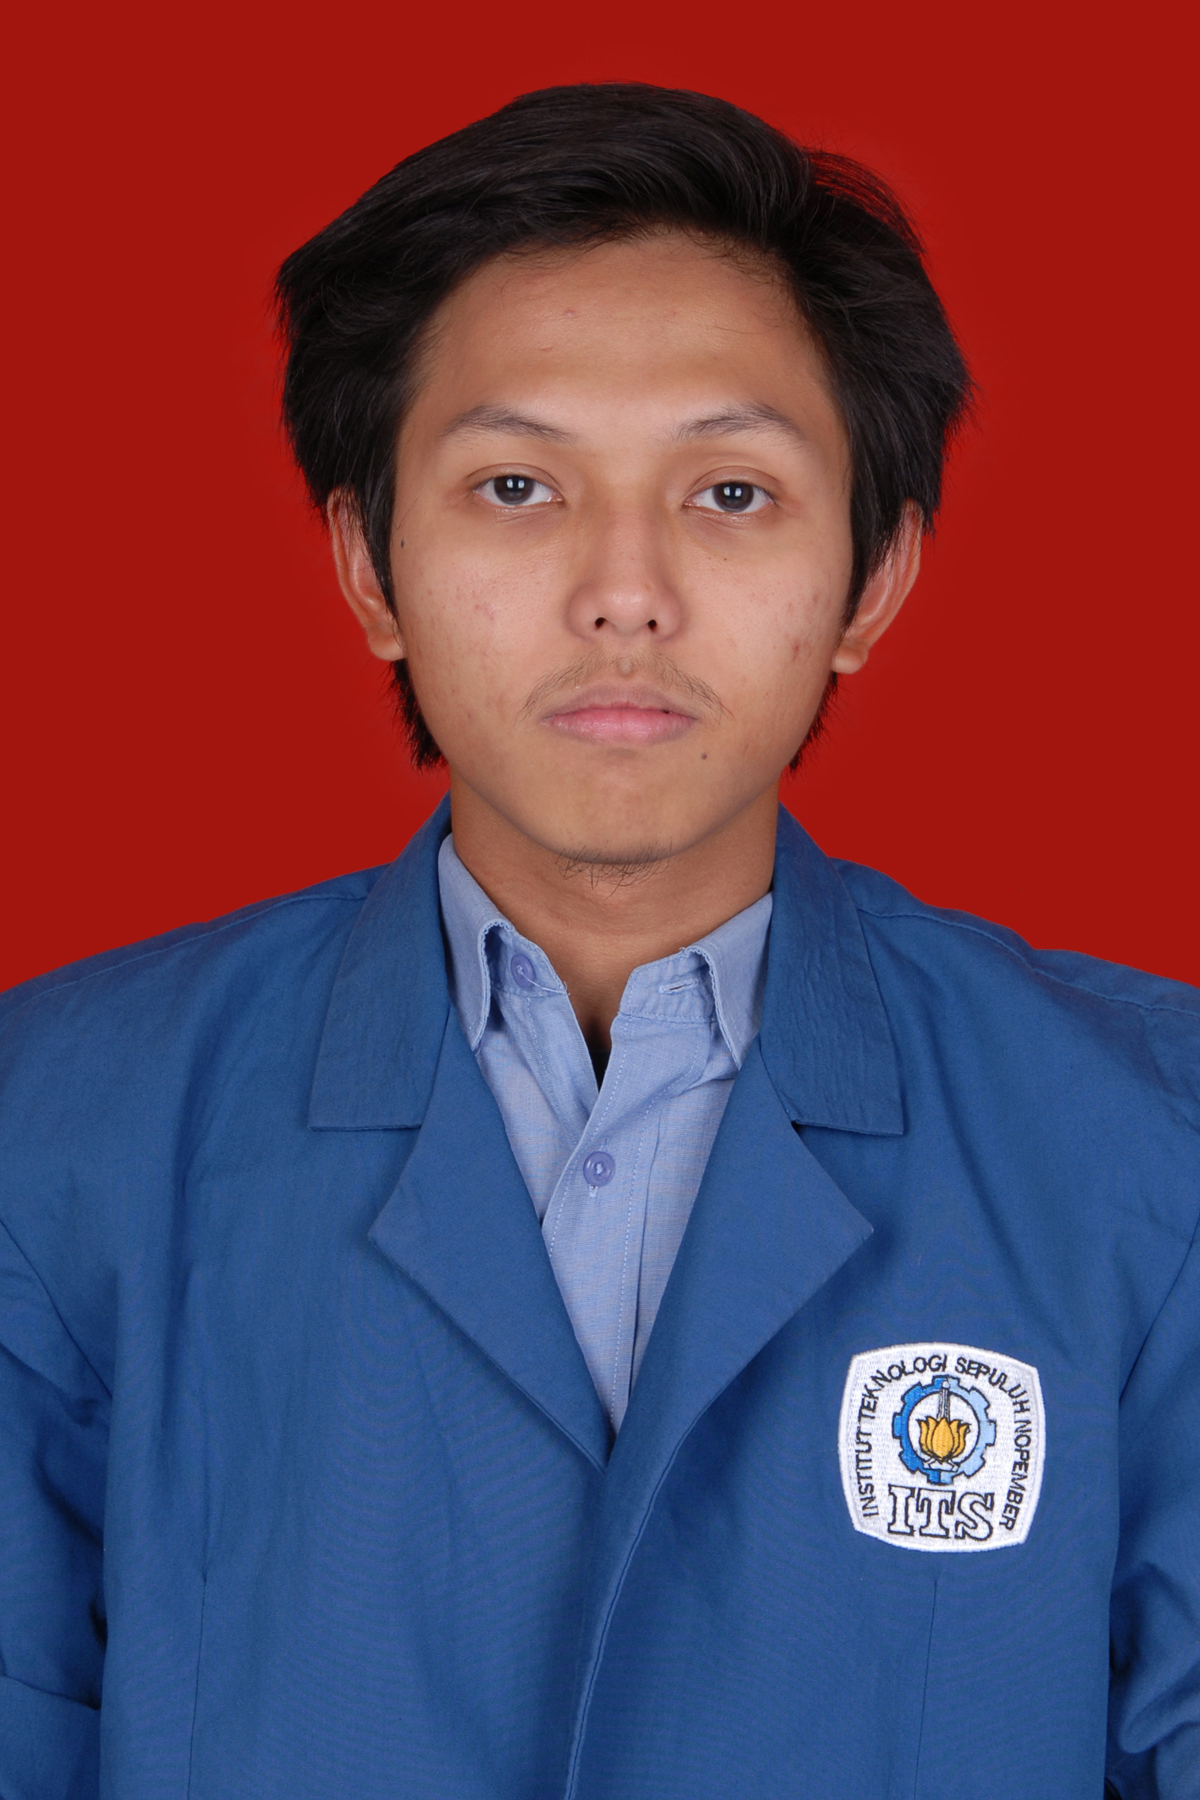
\includegraphics[width=0.29\textwidth]{images/cover/pic}
		\end{wrapfigure}
		Fourir Akbar, lahir pada tanggal 25 April 1996 di Surabaya. Penulis merupakan seorang mahasiswa yang sedang menempuh studi di Departemen Informatika Institut Teknologi Sepuluh Nopember. Memiliki beberapa hobi antara lain futsal dan DOTA. Pernah menjadi asisten dosen pada mata kuliah sistem operasi dan mata kuliah jaringan komputer sebanyak dua semester dan pernah menjadi asisten dosen pada mata kuliah sistem terdistribusi sebanyak satu semester. Penulis juga pernah menjadi asisten dosen pendidikan informatika dan komputer terapan (PIKTI) ITS sebanyak empat semester. Selama menempuh pendidikan di kampus, penulis juga aktif dalam organisasi kemahasiswaan, antara lain sebagai Staff Departemen Hubungan Luar Himpunan Mahasiswa Teknik Computer-Informatika pada tahun ke-2. Penulis juga aktif dalam kepanitiaan Schematics, antara lain sebagai Staff Biro Revolutionary Entertainment and Expo with Various Arts pada tahun ke-2 dan menjadi Badan Pengurus Harian (BPH) Biro Perlengkapan dan Transportasi pada tahun ke-3. Penulis juga merupakan salah satu administrator aktif pada Laboratorium Arsitektur dan jaringan Komputer di Departemen Informatika ITS.
\end{document}